\documentclass[11pt]{article}
\usepackage[T1]{fontenc}
\usepackage[margin=1in]{geometry}
\emergencystretch=2em
\usepackage{amsmath,amssymb,amsthm}
\usepackage{booktabs}
\usepackage{graphicx}
\usepackage{xcolor}
\usepackage{multirow}
\usepackage{algorithm}
\usepackage{algpseudocode}
\usepackage{enumitem}
\usepackage[hidelinks]{hyperref}

\newtheorem{theorem}{Theorem}
\newtheorem{proposition}{Proposition}
\newtheorem{corollary}{Corollary}
\theoremstyle{remark}
\newtheorem{remark}{Remark}

\title{\bf Exact Optimal Transport via the Blossom Algorithm:\\
Benchmarks, Duality Certificates, and a Multi-Robot Application}

\author{
Dmitry Kamenetsky\quad\textit{and}\quad AI Assistant\\
\small{\texttt{dkamenetsky@gmail.com}} \qquad
\small{Arena.ai Agent Mode (autonomous software agent)}
}

\date{\today}

\begin{document}
\maketitle

{\centering\small\itshape
All of the work reported in this paper---algorithm design, implementation,
experiments, analysis, and writing---was performed by the AI agent under the
direction of D.~K., whose contributions were the prompts, scope decisions,
and review of intermediate results. A summary of the prompts used to direct
the work is given in Appendix~\ref{app:prompts}.
\par\vspace{8pt}\par}

\begin{abstract}
Balanced discrete optimal transport between $n$ sources and $n$ targets of
unit mass is, exactly, the minimum-cost assignment problem, i.e.\ a
bipartite perfect matching---so it is solvable \emph{exactly} with the
industrial Blossom engine in milliseconds to seconds. We study when this
exact approach beats the standard approximate alternatives, entropic
Sinkhorn iteration and its state-of-the-art accelerated variant Greenkhorn,
and we make the sparse-exact side \emph{certified}. Three contributions.
(i)~\emph{Measurement}: on dense 2-D instances, exact matching is faster
\emph{and} strictly more accurate than either approximate method throughout
the moderate-$n$ regime: $0.01\,\mathrm{s}$ at $n=500$ to $11.5\,\mathrm{s}$
at $n=8000$, where reaching the same $\le 1\%$ quality target takes the
approximate baselines $12$--$102\,\mathrm{min}$ by measurement-based
extrapolation (factors of $533$--$72{,}000\times$). Greenkhorn, measured
rather than assumed, is $1.0$--$5.0\times$ faster than plain Sinkhorn and
converges to the identical entropic plan, so the quality gap is a
regularization bias shared by both. (ii)~\emph{Theory}: a rigorous gap
certificate for the $k$NN-pool solver that never solves the dense problem:
the pool matching dual returned by Blossom is repaired to dense feasibility
in one $O(n^2)$ pass, yielding a lower bound (Proposition~\ref{prop:repair},
Theorem~\ref{thm:cert}); an entropic dual value provides a second floor
(Theorem~\ref{thm:ent}). On 15 instance families and $k\in\{16,32,64\}$ the
certificate invariants hold on $45/45$ cells; the certified width is
$\le 0.70\%$ at $k=32$ on uniform instances (true gap $\le 0.13\%$) and
tightens monotonically in $k$ on every family. (iii)~\emph{Application}:
multi-robot task allocation, where the discrete plan itself is the
deliverable: per-round exact assignment costs $0.1$--$68\,\mathrm{ms}$,
while a Sinkhorn-plus-hardening pipeline costs $0.12$--$15.9\,\mathrm{s}$
\emph{and} compounds to $+6$--$37\%$ in total travel distance. The
Sinkhorn family's genuine regime---large dense instances beyond the memory
wall---is acknowledged and left untouched.
\end{abstract}

\section{Introduction}
\label{sec:intro}

Discrete optimal transport (OT) is a standard tool in machine learning,
statistics, imaging, and robotics \cite{peyre2019, survey2025}. The scalable
default for large instances is entropic regularization \cite{cuturi2013}:
the smooth problem is solved by the Sinkhorn iteration
\cite{sinkknopp1967}, and---for speed---by accelerated coordinate variants
such as Greenkhorn \cite{awr2017}. Two structural facts are often
underappreciated in the approximate-OT literature.

\begin{enumerate}[leftmargin=2em,itemsep=1pt]
\item \textbf{Balanced unit-mass discrete OT \emph{is} the assignment
problem.} With $n$ sources and $n$ targets of unit mass, a transport plan is
a doubly stochastic matrix and the optimum is attained at a permutation
matrix (Birkhoff--von Neumann; Proposition~\ref{prop:int}). The problem is
therefore a bipartite minimum-weight perfect matching---a special case of
the classical assignment problem \cite{schrijver2003}, solvable exactly by
shortest-augmenting-path methods \cite{jonker1987} and, in its general
(non-bipartite) form, by Edmonds' Blossom algorithm \cite{edmonds1965} as
implemented in the production engines Blossom~V~\cite{blossomv} and
VI~\cite{blossomvi}. Blossom~VI subsumes the bipartite case and is used here
because the same edge-list driver handles arbitrary sparse matchings; exact
solvers return the \emph{optimal integer plan} and its exact value.
\item \textbf{Exact matching is fast.} On the 2-core/2-GB testbed of this
study, dense exact assignment takes $0.01\,\mathrm{s}$ at $n=500$ and
$11.5\,\mathrm{s}$ at $n=8000$; exploiting local structure, a $k$NN-pool
sparse solve takes $0.18\,\mathrm{s}$ at $n=2000$ with a $0.032\%$ gap to
the dense optimum; 1-D instances reach $n=10^6$ in $0.11\,\mathrm{s}$.
\end{enumerate}

The question this paper answers is empirical: \emph{when does exact
matching beat approximate OT?} We answer with (a) a measurement study in
which the approximate baselines---including the state-of-the-art
Greenkhorn---are \emph{implemented and measured, not assumed}; (b) a
\emph{duality certificate} for the pool solver, so that a sparse solution
comes with a rigorous, cheaply computable bound on its distance from the
dense optimum; and (c) an \emph{application hook} in which the discrete
plan is the deliverable (multi-robot task allocation), showing that there
approximation is a tax on both time and quality.

\paragraph{Contributions.}
\begin{enumerate}[leftmargin=2em,itemsep=1pt]
\item A measured comparison of exact matching (dense LAPJV-style Jonker--Volgenant,
  sparse Blossom~VI pool, 1-D closed form) against vanilla Sinkhorn and
  Greenkhorn on dense, clustered, and 1-D+noise instances,
  $n\in\{500,\dots,8000\}$, multiple seeds and distributions
  (Sections~\ref{sec:setup}--\ref{sec:results}).
\item A rigorous \emph{gap certificate} for the pool solver requiring no
  dense solve: a one-sided $O(n^2)$ repair of the pool matching dual to a
  dense-feasible dual (Proposition~\ref{prop:repair},
  Theorem~\ref{thm:cert}), combined with an entropic dual floor
  (Theorem~\ref{thm:ent}). Valid on $45/45$ measured cells;
  $\le 0.70\%$ certified width at $k=32$ on uniform instances; monotone in
  $k$ on every instance (Section~\ref{sec:cert}, Section~\ref{sec:results}).
  The repair is the same clipping operation used for reduced-cost filtering
  in integer programming, but applied here as a stand-alone certificate for
  a $k$NN-pool OT solve; its empirical behaviour is documented across
  families.
\item A multi-robot task-allocation study quantifying the ``discrete plan is
  the deliverable'' regime: exact is millisecond-fast; the approximate
  pipeline is $100$--$240\times$ slower per round and $+6$--$37\%$ worse in
  travel distance (Section~\ref{sec:app}).
\item All code, data, and results are open artifacts under an MIT license
  (Appendix~\ref{app:repro}).
\end{enumerate}

\paragraph{Positioning and related work.}
We do not claim to beat near-linear-time Sinkhorn-family variants on large
dense instances ($n\gg 10^4$): that regime is genuinely theirs, and our
testbed's $2\,\mathrm{GB}$ memory wall sits at $n\approx 1.2\times 10^4$
anyway. The contribution is to \emph{measure} the boundary in the regime
where exact is affordable, to show the state-of-the-art accelerated
approximation does not cross that boundary (it pays the same regularization
gap as plain Sinkhorn), and to \emph{certify} the sparse-exact alternative
so it can be used with provable guarantees. That balanced discrete OT
reduces to the assignment problem is textbook knowledge
\cite{birkhoff1946,schrijver2003,villani2009,peyre2019}; $k$NN sparsification
is a ubiquitous heuristic in OT practice (see the POT library
\cite{flamary2021pot}, screened Sinkhorn \cite{alaya2019screenkhorn},
sparse/multiscale Sinkhorn \cite{schmitzer2016,schmitzer2019stable}); and
exact solvers have long been used as ground truth. Our contribution is to
package the sparse-exact side with a cheap dual certificate and to
benchmark the exact--approximate crossover directly on the moderate-$n$
regime that most practitioners actually operate in.

\section{Preliminaries}
\label{sec:prelim}

\subsection{Discrete OT as assignment}
Let $C\in\mathbb{R}^{n\times n}_{\ge 0}$ be a cost matrix. Write
\[
\mathcal{U}(n) \;=\; \{P\in\mathbb{R}^{n\times n}_{\ge 0} : P\mathbf{1}=\mathbf{1},\;
P^{\mathsf T}\mathbf{1}=\mathbf{1}\}
\]
for the set of feasible plans (each row and column sums to one; total mass
$n$). The discrete transport problem is
\[
\operatorname{OPT}(C) \;=\; \min_{P\in\mathcal{U}(n)} \; \langle C,P\rangle
\;=\; \sum_{i,j} C_{ij}P_{ij}.
\]
We use the total-mass ($n$) convention throughout, so that at an optimum
$\langle C,P\rangle$ is the sum of $n$ edge costs---the assignment cost.
(Readers comparing to references that use the unit-mass convention should
divide our reported costs by $n$.)

\begin{proposition}[OT = assignment; integer optimum]
\label{prop:int}
$\operatorname{OPT}(C)$ is attained at a permutation matrix. Equivalently,
discrete balanced unit-mass OT is the minimum-cost perfect matching in the
complete bipartite graph with edge weights $C_{ij}$.
\end{proposition}
\begin{proof}
By the Birkhoff--von Neumann theorem \cite{birkhoff1946},
$\mathcal{U}(n)$ is the convex hull of the permutation matrices. The
objective $\langle C,\cdot\rangle$ is linear, so its minimum over the
polytope is attained at an extreme point, i.e.\ at a permutation matrix.
Equivalently, the constraint matrix of the transportation problem is
totally unimodular \cite{schrijver2003}. Under any bijection $\pi$, the
permutation matrix $P_{i,\pi(i)}=1$ is a perfect matching of the bipartite
graph with cost $\sum_i C_{i,\pi(i)}$, which proves the equivalence.
\end{proof}

\subsection{Entropic regularization and the Sinkhorn iteration}
For $\varepsilon>0$ define the regularized problem
\begin{equation}
\label{eq:weps}
W(\varepsilon) \;=\; \min_{P\in\mathcal{U}(n)}
\bigl[\,\langle C,P\rangle \;+\; \varepsilon \sum_{ij} P_{ij}\log P_{ij}\,\bigr],
\qquad (0\log 0 := 0).
\end{equation}
The minimizer is the Gibbs kernel $P^{\varepsilon}_{ij}\propto
\exp(-C_{ij}/\varepsilon)$ renormalized to have unit marginals. The
Sinkhorn--Knopp iteration \cite{sinkknopp1967, cuturi2013} alternates row
and column scaling of $K=\exp(-C/\varepsilon)$; in log form, with
potentials $(u,v)$, each pass sets
$P_{ij}=\exp\bigl((u_i+v_j-C_{ij})/\varepsilon\bigr)$ and updates
$u_i\leftarrow u_i - \varepsilon\log(\sum_j P_{ij})$ (columns symmetrically).
We run the log-domain variant, stopping at maximum marginal deviation
$\le 10^{-9}$ or on a cost plateau.

\textbf{Sign convention.}
Equation~\eqref{eq:weps} uses the \emph{negative-entropy} regularizer
$+\varepsilon\sum P_{ij}\log P_{ij}$ (not the more common Shannon form
$-\varepsilon H(P)$ used in \cite{cuturi2013,peyre2019}). Under our
convention $W(\varepsilon)\le\operatorname{OPT}(C)$ (Theorem~\ref{thm:ent});
under the Shannon convention the inequality reverses and $W(\varepsilon)$
is an upper bound. Algorithm~\ref{alg:sink} returns the value consistent
with \eqref{eq:weps}.

Greenkhorn \cite{awr2017} replaces the cyclic pass by a greedy
single-coordinate update: each step picks the most-violated row or column
(measured by a KL-type residual) and applies the exact closed-form update
that restores that one marginal, at $O(n)$ cost per step with incremental
marginal bookkeeping (Algorithm~\ref{alg:green}). The total-work guarantee
of \cite{awr2017} is $\tilde O(n^2/\varepsilon^2)$ (with $O(n)$ per greedy
step), giving a dimension-free dependence in terms of the desired additive
accuracy.

\subsection{Exact solvers used}
\paragraph{Dense.} We use SciPy's optimized Jonker--Volgenant-style
shortest-augmenting-path implementation \texttt{linear\_sum\_assignment}
\cite{jonker1987}, with $\Theta(n^3)$ worst-case time and $O(n^2)$ memory on
dense inputs.
\paragraph{Sparse pool.} For a pool $E_k\subseteq [n]\times[n]$ (the $k$
nearest targets of each source, both sides), solve the assignment
restricted to $E_k$ as a minimum-weight perfect matching with our
edge-list driver for Blossom~VI \cite{blossomvi} (Blossom~V
\cite{blossomv} gives identical costs; see \S\ref{sec:setup}). Costs are
integer (milliunits) as required by the driver. Blossom returns blossom
duals in addition to node potentials; on bipartite inputs the blossom
duals are zero at the optimum, so we restrict to the node potentials
$(\alpha,\beta)$ without loss.
\paragraph{1-D.} If sources and targets lie on a line, the optimal map is
the quantile (order) map (Proposition~\ref{prop:1d}); no matrix is formed.

\begin{proposition}[1-D optimality of the quantile map]
\label{prop:1d}
Let $x_{(1)}\le\cdots\le x_{(n)}$, $y_{(1)}\le\cdots\le y_{(n)}$. For the
quadratic cost (and, more generally, for any convex function $h$, the cost
$h(x_i-y_j)$), the identity map $x_{(i)}\mapsto y_{(i)}$ minimizes
$\sum_i C_{i,\pi(i)}$ over all bijections $\pi$.
\end{proposition}
\begin{proof}
It suffices to show no crossing is present in an optimal map. Suppose
$\pi$ has a crossing: $i<i'$ with $\pi(i)>\pi(i')$. With
$a=x_{(i)}\le b=x_{(i')}$ and $c=y_{\pi(i')}\le d=y_{\pi(i)}$, the
convexity of $h$ gives the Monge inequality
\[
h(a-c)+h(b-d) \;\le\; h(a-d)+h(b-c),
\]
so uncrossing the pair does not increase the cost. Repeated uncrossing
reduces the number of inversions and terminates at the identity map, which
is therefore optimal. \cite[Ch.~2]{villani2009}
\end{proof}

\section{Approximate baselines: implementation and validation}
\label{sec:approx}

Both approximate methods are implemented in the log domain (NumPy,
single-threaded) and stopped at the same marginal tolerance
($10^{-9}$) or, when the cost stagnates (all Greenkhorn cells at the
measured $f$), on a plateau. The regularization is parameterized as a
fraction of the mean cost, $f=\varepsilon/\overline{C}$, on the grid
$f\in\{0.05,0.02,0.01\}$ (plus $0.005$ at $n=500$).

Two validation facts structure the comparison. \emph{First}, Greenkhorn and
vanilla Sinkhorn converge to the \emph{identical} entropic plan up to the
stated stopping tolerance at every measured $(n,f)$ (cost agreement
$\le 0.04\%$, Table~\ref{tab:ghead}), so the comparison between them is
purely a wall-time comparison; the gap to exact is the \emph{regularization
bias}, common to both. \emph{Second}, a Sinkhorn plan is fractional; where
an integer plan is required it must be \emph{hardened} (e.g.\ the
row-argmax permutation, our \texttt{greedy\_hard}). Hardening a converged
$n=500$, $f=0.01$ plan (gap $5.4\%$) costs $+10.9\%$ over the exact
optimum---which the exact solver returns, optimally, in $0.01\,\mathrm{s}$.

\section{Duality certificates for the pool solver}
\label{sec:cert}

This section is the theoretical contribution: a rigorous certificate for
the pool solver that requires \emph{no} dense solve.

\paragraph{Setup.} The pool solver returns a perfect matching $M$ inside
$E_k$, with cost $\mathrm{UB}=\sum_{(i,j)\in M} C_{ij}$. Since $M$ is a
feasible dense solution, $\mathrm{OPT}\le \mathrm{UB}$; $\mathrm{UB}$ is a
trivial upper bound. What a certificate must supply is a lower bound
$\mathrm{LB}\le\mathrm{OPT}$ that is \emph{cheap and rigorous}. Blossom~VI
returns, together with the pool matching, the dual of the pool problem:
node potentials $(\alpha_i,\beta_j)$ with
$\alpha_i+\beta_j\le C_{ij}$ on pool edges and
$\sum_i\alpha_i+\sum_j\beta_j=\mathrm{UB}$ (complementary slackness; the
blossom duals vanish for bipartite instances, see \S\ref{sec:prelim}).
The dual is \emph{not} feasible for the dense problem (it may violate
$\alpha_i+\beta_j\le C_{ij}$ off the pool), so it is not by itself a lower
bound on $\mathrm{OPT}$. The repair below fixes exactly that.

\begin{proposition}[One-sided dual repair]
\label{prop:repair}
Let $(\alpha,\beta)$ satisfy $\alpha_i+\beta_j\le C_{ij}$ for
$(i,j)\in E_k$. Define
\[
\hat\beta_j \;=\; \min\Bigl(\beta_j,\; \min_i \bigl[C_{ij}-\alpha_i\bigr]\Bigr),
\qquad
\hat\alpha_i \;=\; \min\Bigl(\alpha_i,\; \min_j \bigl[C_{ij}-\beta_j\bigr]\Bigr).
\]
Then both $(\alpha,\hat\beta)$ and $(\hat\alpha,\beta)$ are dual-feasible
for the \emph{dense} assignment problem:
$\alpha_i+\hat\beta_j\le C_{ij}$ and $\hat\alpha_i+\beta_j\le C_{ij}$ for
\emph{all} $(i,j)\in[n]^2$.
\end{proposition}
\begin{proof}
Fix any pair $(i,j)$. By definition,
$\hat\beta_j\le C_{ij}-\alpha_i$, since $i$ is one of the indices over
which the inner minimum is taken. Hence
$\alpha_i+\hat\beta_j\le C_{ij}$ for all $(i,j)$. The second statement is
symmetric. $\square$
\end{proof}

\begin{theorem}[Pool gap certificate]
\label{thm:cert}
Let $\mathrm{UB}$ be the pool matching cost and set
\begin{equation}
\label{eq:lb1}
\mathrm{LB}_1 \;=\; \max\Bigl(
\textstyle\sum_i\alpha_i+\sum_j\hat\beta_j,\;\;
\sum_i\hat\alpha_i+\sum_j\beta_j
\Bigr).
\end{equation}
Then $\mathrm{LB}_1\le \mathrm{OPT}(C)\le \mathrm{UB}$, and the pool
solution is certified to be within $\mathrm{UB}-\mathrm{LB}_1$ in absolute
terms (relative width $(\mathrm{UB}-\mathrm{LB}_1)/\mathrm{UB}$, and
$(\mathrm{UB}-\mathrm{LB}_1)/\mathrm{LB}_1$ when $\mathrm{LB}_1>0$) of the
dense optimum---without solving the dense problem.
\end{theorem}
\begin{proof}
By Proposition~\ref{prop:repair}, both repaired pairs are dense dual
feasible; by weak duality for the assignment LP \cite{schrijver2003}, each
of their objectives is a lower bound on $\mathrm{OPT}(C)$, hence so is
their maximum. The upper bound $\mathrm{OPT}\le\mathrm{UB}$ holds because
the pool matching is a feasible dense solution. The gap statements are
immediate algebra from $\mathrm{LB}_1\le\mathrm{OPT}\le\mathrm{UB}$.
\end{proof}

\begin{corollary}
\label{cor:gap}
The certified width is never smaller than the true gap:
$(\mathrm{UB}-\mathrm{LB}_1)/\mathrm{UB}\;\ge\;(\mathrm{UB}-\mathrm{OPT})/\mathrm{UB}$.
The certificate can be loose; it is never wrong.
\end{corollary}

\begin{remark}[Ordering of the repair]
\label{rem:order}
The two one-sided repairs are not comparable in general. The sequential
two-pass variant (clip one side, then clip the other against the \emph{clipped}
first side) is dominated by the one-sided variant that clips the second
side last, but it can underperform the \emph{other} one-sided variant:
on our instances the max-of-two rule of \eqref{eq:lb1} is
$1$--$6\times$ tighter than either single ordering at $k=16$ on structured
instances (e.g.\ $122.7\%\to 12.0\%$ certified width on a 1-D+noise
$n=2000$ instance). We therefore always use \eqref{eq:lb1}.
\end{remark}

\begin{theorem}[Entropic dual floor]
\label{thm:ent}
For every $\varepsilon>0$, $W(\varepsilon)\le \mathrm{OPT}(C)$. In
particular, the value of a \emph{converged} entropic solve,
$V=\langle C,P^{\varepsilon}\rangle+\varepsilon\sum_{ij}P^{\varepsilon}_{ij}
\log P^{\varepsilon}_{ij}$, is a rigorous lower bound on the unregularized
optimum.
\end{theorem}
\begin{proof}
For $x\in[0,1]$ one has $x\log x\le 0$ (with $0\log 0:=0$), and every
entry of $P\in\mathcal{U}(n)$ lies in $[0,1]$ (row sums are one). Hence for
every feasible $P$,
\[
\langle C,P\rangle+\varepsilon\sum_{ij}P_{ij}\log P_{ij}
\;\le\; \langle C,P\rangle .
\]
Taking the minimum over $P\in\mathcal{U}(n)$ gives
$W(\varepsilon)\le \min_P\langle C,P\rangle=\mathrm{OPT}(C)$. A converged
Sinkhorn run satisfies $V=W(\varepsilon)$ up to the duality gap of the
smooth convex problem, which is $0$ at the optimum.
\end{proof}

\begin{remark}[Numerical feasibility]
\label{rem:num}
Our runs stop at maximum marginal deviation $\delta=10^{-9}$, so $P$ is
$\delta$-feasible rather than exactly feasible. A standard feasibility
restoration (add a correction $\Delta$ with $\lVert\Delta\rVert_1\le 2n\delta$)
changes the value by at most
$\lVert C\rVert_\infty\lVert\Delta\rVert_1+O(\varepsilon n\delta)
\;\le\; \lVert C\rVert_\infty\cdot 2n\delta + O(\varepsilon n\delta)$.
On our instances $\lVert C\rVert_\infty\le 141.5$ and $n\le 2000$, so the
correction is $\lesssim 6\times 10^{-4}$ in absolute terms against costs of
$O(10^3)$---nine orders of magnitude below any gap reported.
\end{remark}

\paragraph{Combined certificate.} We report
$\mathrm{LB}=\max(\mathrm{LB}_1,\, W(\varepsilon))$ with
$\varepsilon=0.05\,\overline{C}$ whenever the Sinkhorn run converges in
time. In every measured instance the dual-repair bound $\mathrm{LB}_1$
dominates the entropic one at $k\ge 16$. At the affordable
$\varepsilon=0.05\overline{C}$ the entropy term
$\varepsilon\sum P^\varepsilon_{ij}\log P^\varepsilon_{ij} \approx
-\varepsilon n\log n$ is large and negative (for $n=2000$, $\varepsilon\approx 3.5$,
on the order of $-5\times 10^4$), which makes $W(\varepsilon)$ a valid but
\emph{vacuous} lower bound---negative on most families and far below $\mathrm{LB}_1$.
$W(\varepsilon)$ becomes tight only when $\varepsilon$ is small enough
that Sinkhorn itself is more expensive than the dense solve. We therefore
report $\mathrm{LB}_2=W(\varepsilon)$ only as a labelled cross-check; the
certificate's real work is done by $\mathrm{LB}_1$.

\section{Experimental setup}
\label{sec:setup}

\paragraph{Testbed.} 2-core / 2-GB sandbox; single-threaded Python 3.13
with NumPy and SciPy's Jonker--Volgenant-style assignment routine for the
dense exact, Sinkhorn, and Greenkhorn codes; a C++20 build of Blossom~VI
\cite{blossomvi} (edge-list driver, integer milliunit costs) for the pool
solves; and Blossom~V \cite{blossomv}, used only to cross-validate
matching costs (identical on every instance tested). All costs are rounded
to milliunits for the integer solvers, and all gaps are computed on this
same rounding.

\paragraph{Instance families} (2-D Euclidean distances; details in
Appendix~\ref{app:detail}).
\begin{itemize}[leftmargin=2em,itemsep=1pt]
\item \textbf{uniform}: i.i.d.\ points in $[0,100)^2$.
\item \textbf{clustered}: 8 cluster centers in $[0,100)^2$; each side's
  points are assigned round-robin to a center with Gaussian noise
  ($\sigma=8$); the two sides share the assignment, with the target centers
  jittered by isotropic Gaussian noise of standard deviation $3$
  (i.e.\ $\mathcal{N}(0,3^2 I)$)---corresponding Gaussian clusters.
\item \textbf{1-D+noise}: one-dimensional points on two parallel noisy
  lines (position noise $\sigma=2$; cross noise $\sigma=2$)---a near-Monge
  structure with disorder.
\end{itemize}
Dense grid: $n\in\{500,1000,2000,4000,8000\}$, seed 7, uniform
($n=12000$ OOMs: the $1.15\,\mathrm{GB}$ cost matrix alone exceeds the
2-GB budget). Robustness sweep: $n=1000$, seeds 7--10, all three families
(9 configurations); certificate study adds $n=2000$, seed 7, all families
(15 configurations in total). The multi-robot application uses
$n\in\{50,200,800\}$, seeds 7--8, 15 rounds.

\section{Results}
\label{sec:results}

\subsection{Dense scaling: exact is cheap}
Table~\ref{tab:dense} reports dense exact costs and times (uniform, seed 7).
The $n^3$ law holds cleanly to $n=8000$; $n=12000$ is the memory wall.

\begin{table}[t]
\centering
\begin{tabular}{rrr}
\toprule
$n$ & exact cost & $t(\mathrm{exact})$ \\
\midrule
500  & 2064.1  & 0.01\,s \\
1000 & 3107.0  & 0.06\,s \\
2000 & 4146.4  & 0.23\,s \\
4000 & 6963.2  & 2.16\,s \\
8000 & 10873.4 & 11.48\,s \\
\bottomrule
\end{tabular}
\caption{Dense exact assignment (Jonker--Volgenant), uniform seed 7.
  Costs use the total-mass convention; divide by $n$ for the per-unit-mass
  value common in the OT literature.}
\label{tab:dense}
\end{table}

\subsection{The quality--time trade-off of the approximate methods}
Table~\ref{tab:approx} reports vanilla Sinkhorn on the dense grid. Two
features stand out. \emph{(i) The gap is a regularization bias:}
an ordinary least-squares linear fit through the origin on the three
converged $n=500$ points $f\in\{0.01,0.02,0.05\}$ (gaps
$5.42\%$, $15.02\%$, $58.41\%$) gives slope $m\approx 1353$, i.e.\
gap $\approx 1353\,f$ per cent. The gap/$f$ ratio itself increases with
$f$, so the linear form is an approximation. \emph{(ii) At fixed $f$ the
gap \emph{grows} with $n$:} $15.02\%\to 24.19\%\to 43.78\%$ at $f=0.02$
for $n=500/1000/2000$.

\begin{table}[t]
\centering
\begin{tabular}{rrrr}
\toprule
$n$ & $f$ & gap \% & $t(\mathrm{Sinkhorn})$ \\
\midrule
500  & 0.05 & +58.41  & 10\,s  \\
500  & 0.02 & +15.02  & 34\,s  \\
500  & 0.01 & +5.42   & 74\,s  \\
500  & 0.005 & +2.09 & 400\,s (capped) \\
1000 & 0.05 & +91.40  & 32\,s  \\
1000 & 0.02 & +24.19  & 111\,s \\
1000 & 0.01 & +8.60   & 221\,s \\
2000 & 0.05 & +159.75 & 130\,s \\
2000 & 0.02 & +43.78  & 400\,s (capped) \\
\bottomrule
\end{tabular}
\caption{Vanilla Sinkhorn (log domain, marginal tolerance $10^{-9}$),
uniform seed 7.}
\label{tab:approx}
\end{table}

\paragraph{The $1\%$ target, rough extrapolation.}
Taking the slope above as the local gap rate, the $1\%$ target would
require $f^*\approx 1/1353\approx 7.4\times 10^{-4}$. A log-log linear
fit to Greenkhorn's step count on the four $n=500$ plateau runs gives
$1.241\times 10^4\,f^{-1.03}$, i.e.\ $\approx 2.13\times 10^7$ steps at
$f^*$; per-step costs are the \emph{measured} ones, scaled in $n$ as $O(n)$
(Greenkhorn) and $O(n^2)$ (vanilla) from the measured runs.
Table~\ref{tab:target} gives the result. These numbers are a \emph{rough
extrapolation} (a power law fitted on four points and projected an order
of magnitude outside the measured range), not a rigorous bound; they are
optimistic for the approximate methods, because at fixed $f$ the gap grows
with $n$ (Table~\ref{tab:approx}), so the $f$ required to hit $1\%$ at
larger $n$ is likely smaller than $f^*$, making these times a lower bound
on the true cost. Even so, the factor over exact is $533\times$--$72{,}000\times$.

\begin{table}[t]
\centering
\begin{tabular}{rrrr}
\toprule
$n$ & $t(\mathrm{exact})$ & $t(\mathrm{Sinkhorn\ at\ }f^*)$ & $t(\mathrm{Greenkhorn\ at\ }f^*)$ \\
\midrule
500  & 0.01\,s  & 227\,min   & 12\,min  \\
1000 & 0.06\,s  & 909\,min   & 15\,min  \\
2000 & 0.23\,s  & 3637\,min  & 25\,min  \\
4000 & 2.16\,s  & 14546\,min & 51\,min  \\
8000 & 11.48\,s & 58184\,min & 102\,min \\
\bottomrule
\end{tabular}
\caption{Wall time to reach the $1\%$ quality target. Approximate times are
  a rough power-law extrapolation described in the text; they are
  optimistic for the approximate methods (see text).}
\label{tab:target}
\end{table}

\subsection{Measured head-to-head: Greenkhorn vs vanilla}
Table~\ref{tab:ghead} is the measured comparison between the two
approximate methods at every $(n,f)$ cell. The SOTA accelerated method
\emph{does not close the gap to exact}: it converges to the identical
entropic plan up to plateau tolerance (cost agreement $\le 0.04\%$) and is
$1.0$--$5.0\times$ faster than plain Sinkhorn on the seven cells where
vanilla converged (six of seven within $1.5\times$; the $5.01\times$
outlier is $n=2000$, $f=0.05$). In this small-regularization,
high-condition-number regime the greedy selection makes less progress per
step than a full cyclic pass and plateaus in marginal accuracy
($10^{-6}$--$10^{-3}$ vs $10^{-9}$) while the gap has already settled.

\begin{table}[t]
\centering
\small
\begin{tabular}{rrrrrrrr}
\toprule
$n$ & $f$ & gap V \% & $t(V)$ s & gap G \% & $t(G)$ s & steps(G) & $t(V)/t(G)$ \\
\midrule
500  & 0.05 & +58.41 & 10  & +58.41 & 10 & 260k  & $0.93\times$ \\
500  & 0.02 & +15.02 & 34  & +15.01 & 27 & 760k  & $1.26\times$ \\
500  & 0.01 & +5.42  & 74  & +5.40  & 52 & 1.48M & $1.45\times$ \\
500  & 0.005 & +2.09 & 400$^\dagger$ & +2.07 & 94 & 2.82M & $4.27\times$ \\
1000 & 0.05 & +91.40 & 32  & +91.40 & 25 & 520k  & $1.28\times$ \\
1000 & 0.02 & +24.19 & 111 & +24.17 & 77 & 1.82M & $1.44\times$ \\
1000 & 0.01 & +8.60  & 221 & +8.56  & 151 & 3.6M  & $1.47\times$ \\
2000 & 0.05 & +159.75 & 130 & +159.75 & 26 & 340k & $5.01\times$ \\
2000 & 0.02 & +43.78 & 400$^\dagger$ & +43.77 & 90 & 1.26M & $4.42\times$ \\
\bottomrule
\end{tabular}
\caption{Vanilla Sinkhorn (V) vs Greenkhorn (G), uniform seed 7.
$^\dagger$ 400\,s cap (vanilla did not converge there). All Greenkhorn runs
stopped on a cost plateau before reaching marginal tolerance $10^{-9}$
(typical plateau $10^{-6}$--$10^{-3}$); cost agreement $\le 0.04\%$ in
every cell.}
\label{tab:ghead}
\end{table}

\subsection{The pool solver and its certificate}
Table~\ref{tab:pool} shows the pool solver on the dense $n=2000$ reference
(quality vs $k$); Figure~\ref{fig:crossover} situates it in the
quality--time plane against the approximate baselines. At small $k$
(e.g.\ $k=4$ on this instance) the pool happened to contain a perfect
matching; at $k=1$ Hall's condition fails and the solver reports
infeasible (Appendix~\ref{app:detail}).

\begin{table}[t]
\centering
\small
\begin{tabular}{rrrrr}
\toprule
$k$ & pool edges & cost & gap vs exact & $t(\mathrm{sparse})$ \\
\midrule
4   & 19{,}973  & 5757.7 & +38.861\% & 0.02\,s \\
8   & 35{,}918  & 4388.6 & +5.842\%  & 0.05\,s \\
16  & 67{,}685  & 4170.5 & +0.581\%  & 0.08\,s \\
32  & 130{,}860 & 4147.7 & +0.032\%  & 0.18\,s \\
64  & 255{,}711 & 4146.5 & +0.003\%  & 0.40\,s \\
256 & 962{,}049 & 4146.4 & +0.000\%  & 1.76\,s \\
\bottomrule
\end{tabular}
\caption{$k$NN-pool exact assignment (Blossom~VI), $n=2000$ uniform seed 7;
dense exact $=4146.4$ in $0.23\,$s. Feasibility at small $k$ is
instance-dependent; at $k=1$ the pool is Hall-infeasible.}
\label{tab:pool}
\end{table}

The certificate study (Section~\ref{sec:cert}) ran all 15 configurations
(seeds 7--10 $\times$ families at $n=1000$; seed 7 at $n=2000$) at
$k\in\{16,32,64\}$: \textbf{45/45 cells satisfy
$\mathrm{LB}\le \mathrm{exact}\le \mathrm{UB}$ and
certified width $\ge$ true gap} (asserted in the study code).
Table~\ref{tab:cert} summarizes the certified width
$(\mathrm{UB}-\mathrm{LB})/\mathrm{UB}$ by family;
Figure~\ref{fig:cert} shows it per configuration.

\begin{table}[t]
\centering
\small
\begin{tabular}{lccc}
\toprule
family (\#configs) & $k=16$ & $k=32$ & $k=64$ \\
\midrule
uniform (5)     & 2.57--6.26\%  & \textbf{0.07--0.70\%} & 0.01--0.02\% \\
clustered (5)   & 5.61--38.25\% & 1.03--21.88\% & 0.17--5.90\% \\
1-D+noise (5)   & 11.94--17.35\% & 1.89--3.59\% & 0.24--0.79\% \\
\midrule
true gaps, $k=16$ / $k=32$ / $k=64$ &
0.52--3.84\% & 0.010--2.60\% & 0.000--1.85\% \\
\bottomrule
\end{tabular}
\caption{Certificate width by family (range over the five configurations
each); all 45 cells carry $\mathrm{LB}>0$.}
\label{tab:cert}
\end{table}

\begin{figure}[t]
\centering
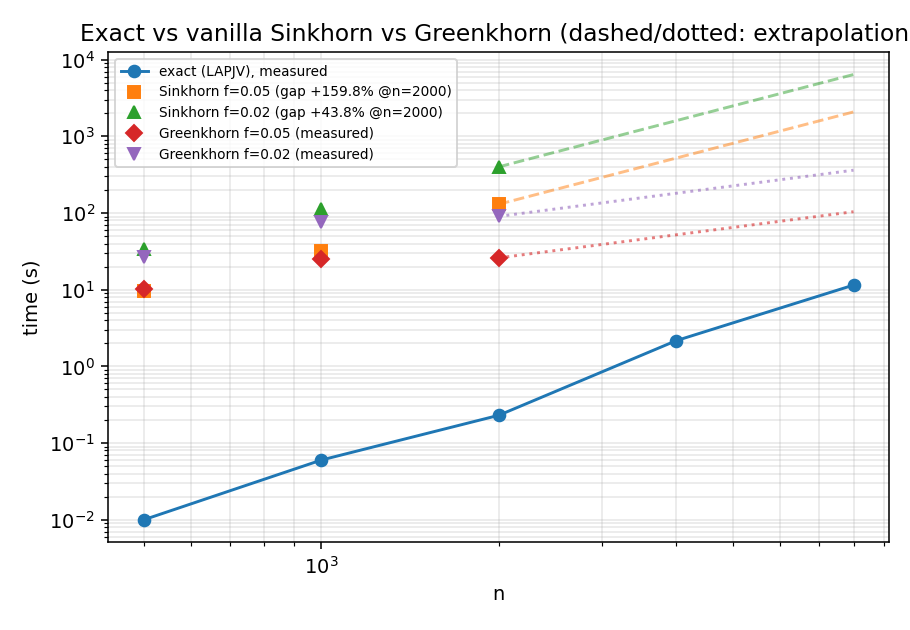
\includegraphics[width=0.98\textwidth]{figs/crossover.png}
\caption{Exact (Jonker--Volgenant) vs vanilla Sinkhorn and Greenkhorn on
the dense uniform grid; dashed/dotted lines are the rough measurement-based
extrapolations to the $1\%$ target. Exact is below both approximate curves
at every measured $n$ in both time and quality.}
\label{fig:crossover}
\end{figure}

\begin{figure}[t]
\centering
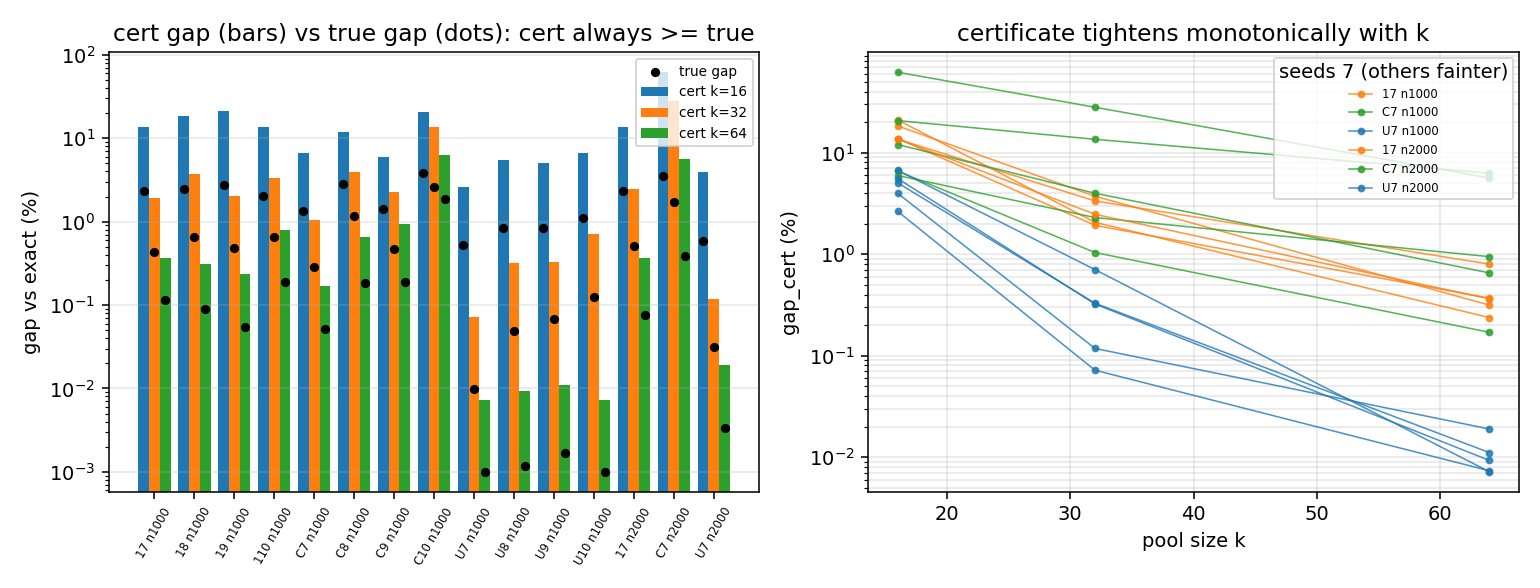
\includegraphics[width=0.98\textwidth]{figs/pool_cert.png}
\caption{Certificate per configuration. Left: certified width (bars) vs
true gap (dots) for $k\in\{16,32,64\}$---the bar is always at or above the
dot. Right: certified width vs $k$, monotone decreasing on every
configuration.}
\label{fig:cert}
\end{figure}

\paragraph{Reading.}
(i)~\emph{Validity}: the certificate is a theorem; the 45/45 check is a
test of the implementation, not of the math. (ii)~\emph{Tightness}: where
the pool is tight (uniform instances), the width is tight too---$\le 0.70\%$
at $k=32$ against a true gap $\le 0.13\%$, and $\le 0.02\%$ at $k=64$.
On the block-structured (clustered) and near-Monge (1-D+noise) families the
repair is conservative: the pool dual is large where it must be clipped
hard against cheap off-pool edges, so the width is looser (up to
$21.88\%$ at $k=32$, true gap $1.73\%$). It is still a \emph{valid} bound,
and---importantly---the width \emph{tightens monotonically in $k$ on every
configuration}, so ``widen the pool'' is a certified escape hatch.
(iii)~\emph{Cost}: certificate $=$ pool solve $+$ one $O(n^2)$ repair,
$\le 0.73\,\mathrm{s}$ in total on our $n=2000$ cells, comparable to the
dense solve.

\subsection{Robustness across seeds and distributions}
On the 9-configuration $n=1000$ sweep (seeds 7--10 $\times$ families):
exact is fastest everywhere ($0.07$--$0.10\,$s) and optimal; the $k=32$
pool solver is feasible in $9/9$ with gaps $+0.010\%$ to $+2.599\%$ in
$<0.15\,$s; Greenkhorn at $f=0.01$ sits at $+6.3\%$ to $+14.7\%$ (agreeing
with vanilla to $\le 0.05\%$ in the 8 converged cells); vanilla needs
$\ge 400\,$s \emph{without converging} on the four symmetric clustered
configurations, where Greenkhorn's plateau matches it in $50$--$98\,$s.

\subsection{1-D structure}
The quantile map solves the 1-D family in $O(n\log n)$ with no matrix:
$n=10^6$ in $0.11\,$s, where the dense cost matrix alone is $8\,\mathrm{TB}$.

\section{Application: multi-robot task allocation}
\label{sec:app}

The clearest regime for the discrete plan as deliverable is multi-robot
task allocation \cite{gerkey2004}: in warehouse picking, drone teaming, or
AMR dispatch, each of $n$ robots must be assigned \emph{exactly one} of $n$
tasks---a fractional transport plan is physically meaningless (one cannot
dispatch half a robot). The standard practice is precisely the
Hungarian/auction family of exact solvers \cite{bertsekas1989, jonker1987}.

\paragraph{Protocol.} Open field $[0,100)^2$; 15 rounds; each round, $n$
fresh tasks appear, robots are (re)assigned with cost
$C_{ij}=\lVert r_i - t_j\rVert_2$ from the robots' current positions, and
robots then move to their tasks. All three policies share the \emph{same}
start positions and the \emph{same} task stream per round, so only the
per-round assignment differs. Policies: \textbf{exact} (Jonker--Volgenant
per round); \textbf{greedy} (cheapest-first); \textbf{Sinkhorn+hardening}
(our $f=0.05$, tolerance $10^{-7}$ pipeline from
Section~\ref{sec:approx}; an integer plan is produced regardless).
$n\in\{50,200,800\}$, seeds 7--8; Table~\ref{tab:robot} reports the
episode totals.

\begin{table}[t]
\centering
\small
\begin{tabular}{rrrrrrr}
\toprule
$n$ & seed & travel (exact) & greedy & Sinkhorn+hard & gap greedy & gap Sinkh. \\
\midrule
50  & 7 & 10232.8 & 12353.3 & 10930.4 & +20.72\% & +6.82\% \\
50  & 8 & 10531.8 & 12357.2 & 11134.9 & +17.33\% & +5.73\% \\
200 & 7 & 21835.6 & 28718.1 & 24955.1 & +31.52\% & +14.29\% \\
200 & 8 & 23804.5 & 30051.8 & 26802.5 & +26.24\% & +12.59\% \\
800 & 7 & 47327.7 & 64986.7 & 59959.2 & +37.31\% & +26.69\% \\
800 & 8 & 49050.9 & 66519.9 & 61229.6 & +35.61\% & +24.83\% \\
\bottomrule
\end{tabular}
\caption{Total travel distance over 15 rounds; gaps relative to the
exact-assignment policy, which is the best achievable (optimal every
round).}
\label{tab:robot}
\end{table}

\begin{figure}[t]
\centering
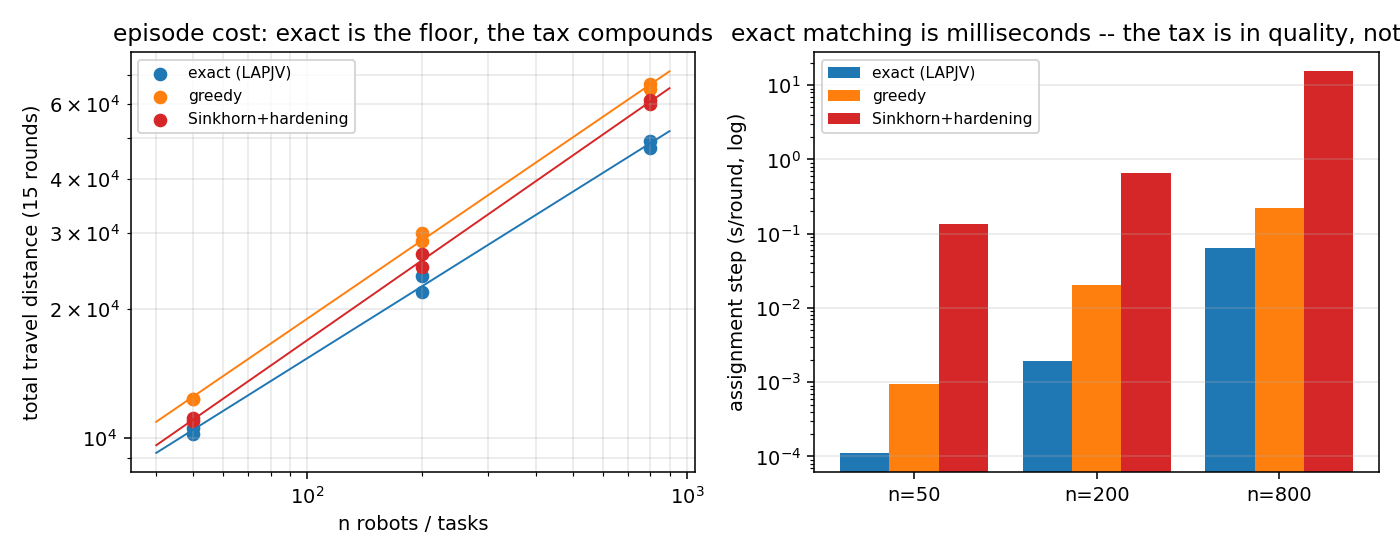
\includegraphics[width=0.98\textwidth]{figs/app_hook.png}
\caption{Left: episode travel distance vs $n$ (the quality tax compounds
with $n$). Right: cost of the assignment step per round (log scale):
exact matching is milliseconds; the Sinkhorn pipeline is $10^2$--$10^3\times$
slower.}
\label{fig:robot}
\end{figure}

\paragraph{Findings.}
(i)~\emph{The quality tax accumulates}: per-round gaps compound through
robot positions; over 15 rounds greedy ends $+17.3$--$+37.3\%$ and
Sinkhorn+hardening $+5.7$--$+26.7\%$ above the exact policy, and the gap
grows with $n$ (the entropic gap grows with $n$ at fixed $f$,
Section~\ref{sec:results}). (ii)~\emph{Approximate is not even faster
here}: the assignment step takes exact $0.1$--$68\,\mathrm{ms}$/round vs
$0.12$--$15.9\,$s for the Sinkhorn pipeline ($\approx 239\times$ at
$n=800$). (iii)~\emph{The hook}: where the discrete plan is the deliverable,
approximate OT is a tax on \emph{both} time and distance at
$n\le 10^3$; the exact default holds up to the memory wall.

\section{Discussion}
\label{sec:disc}

\paragraph{Empirical decision rule.}
Integer plan needed $\to$ exact; 1-D/Monge $\to$ closed form; local/$k$NN
structure $\to$ sparse pool exact, \emph{with its certificate}
(Section~\ref{sec:cert}); dense, no structure, fractional plan
acceptable $\to$ exact up to the memory wall ($n\approx 1.2\times 10^4$
on this hardware), beyond which the Sinkhorn family wins on time and
memory---that regime is genuinely theirs.

\paragraph{Why the certificate matters, and what it is not.}
Pool sparsity is a heuristic; the certificate converts it into a
\emph{guarantee}: the solver announces ``my solution is within $w\%$ of
optimal'' with $w$ computed from its own dual in milliseconds. In
applications where a $\le 1\%$ guarantee is a requirement (dispatching,
pricing, auditing), this replaces a dense re-solve or a conservative
safety margin. Mechanically, the one-sided clip is the same dual restriction
used classically for reduced-cost variable fixing in integer programming
\cite{schrijver2003} and bears a family resemblance to screening tests for
entropic OT \cite{alaya2019screenkhorn}. What distinguishes it here is the
packaging: (a)~the clip runs in a single $O(n^2)$ pass \emph{after} the
sparse solve and requires no iteration; (b)~the max-of-two rule gives a
noticeably tighter bound than either one-sided clip alone
(Remark~\ref{rem:order}); and (c)~it certifies an \emph{exact} pool
solution rather than screening edges for a regularized solver.

\paragraph{Limitations.}
(i) Two-core/2-GB testbed: wall times are single-machine; the memory wall
($n\approx 1.2\times 10^4$) is hardware-specific, though the $O(n^2)$
memory of any dense method is not. (ii) The $f^*$ extrapolation
(Table~\ref{tab:target}) is a rough power-law projection, not a theorem,
as documented. (iii) The certificate is conservative on block-structured
instances (Remark~\ref{rem:order}; Table~\ref{tab:cert}); a
structure-aware repair (e.g.\ exploiting the cluster geometry) is future
work. (iv) The application is synthetic (no obstacles, kinematics, or
traffic); the point is structural---the discrete plan is the deliverable---
not a robotics benchmark. (v) We do not compare against GPU
approximate-matching or near-linear Sinkhorn implementations; those target
exactly the large-$n$ regime we do not claim.

\section{Conclusion}
Balanced discrete OT is the assignment problem, and the assignment problem
is a matching problem---so the industrial Blossom engine gives exact optimal
transport with an integer plan and an exact value. Measured against the
standard approximate alternatives on the moderate-$n$ regime, exact is
faster \emph{and} more accurate; the state-of-the-art accelerated
approximation (Greenkhorn) improves on plain Sinkhorn by $1$--$5\times$ but
pays the same regularization gap. We gave the sparse pool solver a rigorous
gap certificate---a repaired matching dual that costs one $O(n^2)$ pass and
is comparable in cost to the dense solve it certifies---and showed, in a
multi-robot application, that where the plan itself is the deliverable,
approximate OT is a tax on both time and quality. The Sinkhorn family's
large-$n$ dense regime stands untouched, and the boundary between the two
regimes is now measured and certified rather than assumed.

\begin{thebibliography}{20}

\bibitem{edmonds1965}
J.~Edmonds. \emph{Maximum matching and a polyhedron with $0$,$1$-vertices}.
Journal of Research of the National Bureau of Standards, Section~B,
69B:125--130, 1965.

\bibitem{birkhoff1946}
G.~Birkhoff. \emph{Tres observaciones sobre el algebra lineal}.
Anales de la Universidad Nacional de Educaci\'on J.\,P.~Bustos, 1946.

\bibitem{schrijver2003}
A.~Schrijver. \emph{Combinatorial Optimization: Polyhedra and Efficiency}.
Springer, 2003.

\bibitem{jonker1987}
R.~Jonker and A.~Volgenant. \emph{A shortest augmenting path algorithm for
dense and sparse linear assignment problems}. Computing, 38(4):325--340,
1987. (Earlier version in WADS, LNCS~246, Springer, 1987.)

\bibitem{blossomv}
V.~Kolmogorov. \emph{Blossom V: a new implementation of Edmonds' algorithm
for minimum weight perfect matching}. Mathematical Programming Computation,
1(1):43--67, 2009. Code: \url{https://github.com/orkz/BlossomV}.

\bibitem{blossomvi}
G.~Arkhipov and V.~Kolmogorov. \emph{Blossom VI: A Practical Minimum Weight
Perfect Matching Algorithm}. arXiv:2604.20351 (to appear, ALENEX 2027),
2026.

\bibitem{sinkknopp1967}
R.~Sinkhorn and P.~Knopp. \emph{Concerning nonnegative matrices and doubly
stochastic matrices}. Pacific Journal of Mathematics, 22(2):343--348, 1967.

\bibitem{cuturi2013}
M.~Cuturi. \emph{Sinkhorn distances: lightspeed computation of optimal
transport}. Advances in Neural Information Processing Systems 26, 2013.

\bibitem{awr2017}
J.~Altschuler, J.~Weed, and P.~Rigollet. \emph{Near-linear time approximation
algorithms for optimal transport via Sinkhorn iteration}. Advances in
Neural Information Processing Systems 30, 2017. arXiv:1705.09634.

\bibitem{peyre2019}
G.~Peyr\'e and M.~Cuturi. \emph{Computational Optimal Transport}.
Foundations and Trends in Machine Learning, 11(5):355--607, 2019.

\bibitem{survey2025}
S.~Moradi. \emph{A survey on algorithmic developments in optimal transport
problem with applications}. arXiv:2501.06247, 2025.

\bibitem{villani2009}
C.~Villani. \emph{Optimal Transport: Old and New}. Grundlehren 338,
Springer, 2009.

\bibitem{bertsekas1989}
D.~P.~Bertsekas. \emph{The auction algorithm: a distributed relaxation
method for the assignment problem}. Annals of Operations Research,
29:69--104, 1990.

\bibitem{gerkey2004}
B.~P.~Gerkey and M.~J.~Matari\'c. \emph{A formal analysis and taxonomy of
task allocation in multi-robot systems}. International Journal of Robotics
Research, 23(4):493--512, 2004.

\bibitem{christofides1976}
N.~Christofides. \emph{Worst-case analysis of a new heuristic for the
travelling salesman problem}. Technical report, School of Graduate Studies
in Business Administration, Carnegie-Mellon University, 1976.

\bibitem{schmitzer2016}
B.~Schmitzer. \emph{A sparse multiscale algorithm for dense optimal
transport}. Journal of Mathematical Imaging and Vision, 56(2):238--259,
2016.

\bibitem{schmitzer2019stable}
B.~Schmitzer. \emph{Stabilized sparse scaling algorithms for entropy
regularized transport problems}. SIAM Journal on Scientific Computing,
41(3):A1443--A1481, 2019.

\bibitem{alaya2019screenkhorn}
M.~Z.~Alaya, M.~Berar, G.~Gasso, and A.~Rakotomamonjy. \emph{Screening
Sinkhorn algorithm for regularized optimal transport}. Advances in Neural
Information Processing Systems 32, 2019.

\bibitem{flamary2021pot}
R.~Flamary et al. \emph{POT: Python Optimal Transport}.
Journal of Machine Learning Research, 22(78):1--8, 2021.
\url{https://pythonot.github.io}.

\end{thebibliography}

\appendix

\section{Additional proofs and details}
\label{app:proofs}

\subsection{Feasibility restoration for the entropic floor}
\label{app:restoration}
Theorem~\ref{thm:ent} assumes $P$ is exactly feasible. Suppose instead
$P\ge 0$ with $\lVert P\mathbf{1}-\mathbf{1}\rVert_\infty\le\delta$ and
$\lVert P^{\mathsf T}\mathbf{1}-\mathbf{1}\rVert_\infty\le\delta$. Let
$r=P\mathbf{1}-\mathbf{1}$, $c=P^{\mathsf T}\mathbf{1}-\mathbf{1}$
($\mathbf{1}^{\mathsf T}r=\mathbf{1}^{\mathsf T}c$). There exists a matrix
$\Delta$ with $\Delta\mathbf{1}=-r$, $\Delta^{\mathsf T}\mathbf{1}=-c$
(e.g.\ via the transportation problem on the residuals, which is feasible
exactly when $\mathbf{1}^{\mathsf T}r=0$); one may take
$\lVert\Delta\rVert_1\le 2n\delta$ (send each row's excess to a deficit
column). Then $\tilde P=P+\Delta\ge 0$ is feasible for
$\delta\le \min_{ij}P_{ij}$ and
\[
\bigl|\langle C,\Delta\rangle\bigr| \le \lVert C\rVert_\infty
\lVert\Delta\rVert_1 \le \lVert C\rVert_\infty\, 2n\delta,
\]
while the entropy term changes by
$\varepsilon\sum_{ij}(\tilde P_{ij}\log\tilde P_{ij}-P_{ij}\log P_{ij})
= O(\varepsilon n\delta)$, since $x\log x$ has bounded slope on
$[\delta/2,1]$ apart from entries where both $P_{ij},\tilde P_{ij}\le\delta$
(contributing $O(\varepsilon n\delta|\log\delta|)$ in the worst case). With
$\delta=10^{-9}$, $n\le 2000$, $\lVert C\rVert_\infty\le 141.5$ this is
$\lesssim 6\times 10^{-4}$ absolute---negligible against costs of
$O(10^3)$ (Remark~\ref{rem:num}).

\subsection{Worked example of the certificate}
\label{app:example}
Consider
\[
C=\begin{pmatrix}
57&14&33&40\\
36&29&59&11\\
49&40&58&26\\
38&33&53&42
\end{pmatrix}
\]
with the $2$-NN pool (the union of each row's and each column's two
cheapest edges; 10 of the 16 edges). The pool solver returns the matching
of cost $\mathrm{UB}=122$ and the pool dual
$\alpha=(7,18,33,20)$, $\beta=(18,7,26,-7)$, with
$\sum\alpha+\sum\beta=122=\mathrm{UB}$ and
$\alpha_i+\beta_j\le C_{ij}$ on every pool edge.

\emph{The raw dual is not dense-feasible.} On the two off-pool edges,
$\alpha_3+\beta_1=33+18=51>49=C_{31}$ and
$\alpha_3+\beta_3=33+26=59>58=C_{33}$. (Its objective $122$ even exceeds
the dense optimum---infeasible duals can.) The dense optimum is
$\mathrm{OPT}=121$ (true pool gap $0.83\%$).

\emph{Repair.} Option~B (clip the $\alpha$ side against the original
$\beta$): $\hat\alpha_3=\min\bigl(33,\min_j(C_{3j}-\beta_j)\bigr)
=\min(33,\,49-18,\,40-7,\,58-26,\,26+7)=31$; the other $\alpha_i$ need no
clipping (each already satisfies all dense constraints). Objective:
$(7+18+31+20)+(18+7+26-7)=120$. Option~A (clip
the $\beta$ side against the original $\alpha$) gives
$\hat\beta=(16,7,25,-7)$ with objective $119$. Taking the max
(Theorem~\ref{thm:cert}),
\[
\mathrm{LB}=120\;\le\;\mathrm{OPT}=121\;\le\;\mathrm{UB}=122,
\]
so the pool solution is certified within $\frac{122-120}{122}=1.64\%$
(width) of the dense optimum---here computed by hand; in the implementation
it is two $O(n^2)$ min-passes. Note that the two one-sided options
differ ($120$ vs $119$), illustrating Remark~\ref{rem:order}.


\subsection{Monotonicity of the upper bound in $k$}
Since $E_k\subseteq E_{k'}$ for $k\le k'$, every $k$-pool matching is a
valid $k'$-pool candidate, hence
$\mathrm{UB}_{k'}\le \mathrm{UB}_k$; the pool gap is non-increasing in $k$
by definition. The certified width is monotone in $k$ on all 15 measured
configurations (an empirical fact about the \emph{repair}, not a theorem:
the pool dual changes with $k$).

\section{Experimental details}
\label{app:detail}

\subsection{Instance generators}
\begin{itemize}[leftmargin=2em,itemsep=1pt]
\item \textbf{uniform}: $\mathrm{rng}=\texttt{default\_rng(seed)}$; both
  sides $=100\cdot \mathrm{rng.random}((n,2))$.
\item \textbf{clustered}: centers $c_a=100\cdot\mathrm{rng.random}((8,2))$;
  each side assigns point $i$ to center $a=i\bmod 8$ with
  $x_i=c_{a}+\mathcal N(0,8^2 I)$; the target centers are
  $c'_a=c_a+\mathcal N(0,3^2 I)$ with the same assignment (target-center
  jitter $\sigma=3$, matching the description in \S\ref{sec:setup}).
\item \textbf{1-D+noise}: $t_i\sim U[0,100]$;
  $x_i=(t_i+\mathcal N(0,2),\,\mathcal N(0,2))$; independently
  $s_j\sim U[0,100]$ from $\texttt{default\_rng(seed+1000)}$;
  $y_j=(s_j+\mathcal N(0,2),\,\mathcal N(0,2))$.
\end{itemize}

\subsection{Algorithms}
\begin{algorithm}[h]
\caption{Log-domain Sinkhorn (vanilla)}\label{alg:sink}
\begin{algorithmic}[1]
\Require cost $C\in\mathbb R^{n\times n}$, $\varepsilon>0$, tolerance $\tau$
\State $u\leftarrow 0$, $v\leftarrow 0$
\Repeat
  \For{$i=1,\dots,n$}\State $u_i\leftarrow u_i-\varepsilon\,\mathrm{LSE}_j\bigl((v_j-C_{ij})/\varepsilon\bigr)$\EndFor
  \For{$j=1,\dots,n$}\State $v_j\leftarrow v_j-\varepsilon\,\mathrm{LSE}_i\bigl((u_i-C_{ij})/\varepsilon\bigr)$\EndFor
  \State $P_{ij}\leftarrow \exp((u_i+v_j-C_{ij})/\varepsilon)$
\Until $\max_i|(P\mathbf 1)_i-1|+\max_j|(P^{\mathsf T}\mathbf 1)_j-1|\le\tau$ \emph{or cost plateau}
\State \Return $P$, value $\langle C,P\rangle+\varepsilon\sum P_{ij}\log P_{ij}$
\end{algorithmic}
\end{algorithm}

\begin{algorithm}[h]
\caption{Greenkhorn (after \cite[Alg.~4]{awr2017})}\label{alg:green}
\begin{algorithmic}[1]
\Require $K=\exp(-C/\varepsilon)$ (unnormalized), potentials $x,y=0$,
residual metric $\rho(a,b)=b-a+a\log(a/b)$
\State maintain row/column marginals of $A=D(e^x)K D(e^y)$ incrementally
\Repeat
  \State $I\leftarrow\arg\max_i \rho(1,(A\mathbf 1)_i)$;
  $J\leftarrow\arg\max_j \rho(1,(\mathbf 1^{\mathsf T}A)_j)$
  \If{$\rho_I>\rho_J$}\State $x_I\leftarrow x_I+\log(1/(A\mathbf 1)_I)$\Else
  \State $y_J\leftarrow y_J+\log(1/(\mathbf 1^{\mathsf T}A)_J)$\EndIf
  \State update $A$ and the marginals of the touched line ($O(n)$)
\Until marginal tolerance or cost plateau
\end{algorithmic}
\end{algorithm}

\textbf{Hardening} (\texttt{greedy\_hard}): for $i=1,\dots,n$, set
$\pi(i)=\arg\max_j P_{ij}$ among unused columns, removing row $i$ and
column $\pi(i)$ from $P$; the cost is $\sum_i C_{i,\pi(i)}$ (a feasible
integer plan, hence $\ge \mathrm{OPT}$).

\textbf{Pool construction} (\texttt{knn\_pool}): for each source $i$, keep
the $k$ targets with smallest $C_{ij}$ (and symmetrically for each target);
the pool is the union. If the pool has no perfect matching (Hall's
condition fails, e.g.\ $k=1$), the solver reports infeasible.

\textbf{Certificate} (\texttt{pool\_certified}):
UB/perm/dual from \texttt{blossom\_pool\_duals};
$\mathrm{LB}_1$ from Proposition~\ref{prop:repair} (max of the two
one-sided repairs); $\mathrm{LB}_2=W(0.05\,\overline C)$ from one converged
Sinkhorn run per configuration (shared across $k$);
$\mathrm{LB}=\max(\mathrm{LB}_1,\mathrm{LB}_2)$.

\subsection{Parameters}
Marginal tolerance $10^{-9}$ (application hook: $10^{-7}$, the plan is
hardened anyway); time caps $400\,$s (dense grid), $240\,$s (certificate
study Sinkhorn runs); Blossom VI pool timeout $120\,$s (never hit); costs
rounded to milliunits for the integer solvers; all timings single-threaded
wall time, same machine, same process order.

\section{Reproduction}
\label{app:repro}

All code, data, and results are open artifacts under the MIT license,
available at
\url{https://github.com/dimkadimon/OT-Blossom}.
The repository layout:
\begin{verbatim}
ot-study/otlib.py                  # sinkhorn, greenkhorn, exact, pool,
                                   # dual repair, entropic floor, certificate
ot-study/run_ot_study.py           # Part A/B tables -> results/ot_study.md
ot-study/run_greenkhorn_study.py   # A.2b, A.3, Part D -> results/ot_study.md
ot-study/run_pool_cert_study.py    # certificate study (15 x 3 cells)
                                   # -> results/pool_cert.md, asserts invariants
ot-study/app_hook_robots.py        # multi-robot study -> results/app_hook.md
paper/                             # LaTeX source and figs for this paper
\end{verbatim}
Each script caches its results (JSON) and re-renders in seconds; a full
cold re-run takes $\approx 25\,\mathrm{min}$ (Greenkhorn grid),
$\approx 20\,\mathrm{min}$ (certificate study), $\approx 6\,\mathrm{min}$
(application hook) on the testbed. The Blossom~VI binary used for pool
solves is available from its authors \cite{blossomvi}; our driver uses
the edge-list interface with the \texttt{--duals} flag.

\section{Prompts that directed this work}
\label{app:prompts}

This appendix summarizes, in chronological order, the prompts used by
D.~K.\ to direct the work reported here. Prompts marked (verbatim) are
quoted exactly; earlier prompts are paraphrased from the conversation
record because their exact wording was not preserved.

\begin{enumerate}[leftmargin=2em,itemsep=2pt]
\item (paraphrase) Opening question: can the Blossom (matching) algorithm
be used for the TSP, and if so how---setting up the study of Edmonds'
algorithm as a component of TSP algorithms.
\item (paraphrase) Requests to implement and validate a Christofides
heuristic using Blossom for the matching step against exact optima on small
metric instances, and to benchmark the pre-shortcut multigraph.
\item (paraphrase) Request for a head-to-head comparison of Blossom V and
Blossom VI (matching costs and wall times), including on dense complete
graphs.
\item (verbatim, mid-task) ``Actually you can now use Blossom VI'' with a
link to the Blossom VI repository---direction to make Blossom VI the
default engine (retaining Blossom V for the head-to-head).
\item (paraphrase) Follow-up: ``perturb the 2-matching, merge its cycles
into one tour''---with the standing requirement that the merge be efficient
and come close to the optimal tour, and that results be compared to
state-of-the-art methods.
\item (paraphrase) Request for rigorous lower bounds via matching
(2-factor / cycle-cover relaxations) to certificate the gap of the
merge-based tours.
\item (verbatim) ``Where else is Blossom useful?''---advisory question that
produced the shortlist of exact-matching applications, of which optimal
transport was ranked \#1.
\item (verbatim) ``do \#1''---selection of the OT study as the next project.
\item (verbatim) ``Yes build it. Continue clearing the publication bar''---
approval to build the measured SOTA (Greenkhorn) baseline and the seed/distribution
robustness sweep.
\item (verbatim) ``Continue bridging the publication bar''---direction to
complete the remaining two items: a pool solver with a gap certificate,
and an application hook where the discrete plan is the deliverable.
\item (verbatim, this paper) ``excellent! can you prepare an arXiv paper
about it with references and proofs. Make it professional and publishable.
Add an appendix section where you summarise the prompts I have used here.
Can you add me to the author list (Dmitry Kamenetsky with email
dkamenetsky@gmail.com) and the AI. Mention that all the work was done by AI
with the suggestion from me. Also convert it to a pdf so I can look at it''
\end{enumerate}

\end{document}
